\subsection{Resultat}

\subsection{Strategier}
Strategierna har utvecklats utav oss inom gruppen och har under projektets gång ifrågasatts en del. Vissa strategier har upplevts som meningslösa. I efterhand hade vi kunnat låta personer utanför projektgruppen skapa strategier, exempelvis som en tävling för att verkligen finna intressanta strategier, och framför allt fler strategier som tar hänsyn till resultathistoriken.

Grudger är en samarbetande strategi som belönar andra strategier som samarbetar, men straffar strategier som försöker maximera vinsten. Det gör att Grudger får bra poängutdelning mot strategier som också samarbetar(så som tit-for-tat, goog-guy-greg och sig själv). De strategier som försöker maximera sin egen vinst kommer Grudger att straffa genom att bara spela ettor. Det gör att Grudger kommer att erhålla poäng varje omgång så länge inte motståndaren också spelar ettor.  Om Grudger möter en strategi som också straffar sina motståndare så kommer båda dessa strategier att spela ettor. Detta resulterar i att ingen av strategierna kommer att få några poäng eftersom de spelar lika varje omgång. Exempel på detta beteende kan observeras när Grudger möter strategier som den inte lyckas få någon vinst mot så som loler-guy, median-guy med flera.

\begin{figure}[htb]
	\begin{center}
	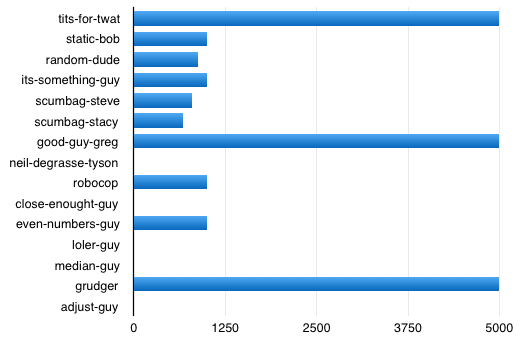
\includegraphics[scale=0.75, angle=0]{bilder/grudger.png}
	\caption{Detta är bildtexten}
	\label{grudger}
	\end{center}
\end{figure}

Den strategi som lyckats best i är tit for tat. I figur * syns det tydligt att tit for tat spelar bra mot majoriteten av de andra strategierna. De strategier som tit for tat har svårt mot är de som tvingar den andra strategin att tillslut bara spela ettor. Mot dessa kommer tit for tat bara att få några få poäng. Mot statiska strategier lyckas tit for tat hitta ett läge där den maximerar sin vinst. Detta gör att den har någorlunda stora vinster mot its something guy, robocop och static Bob.

\begin{figure}[htb]
	\begin{center}
	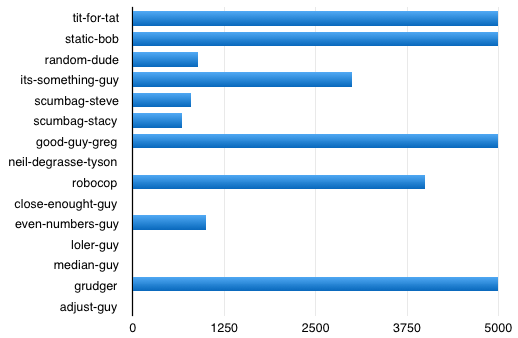
\includegraphics[scale=0.75, angle=0]{bilder/tit-for-tat.png}
	\caption{Detta är bildtexten}
	\label{tit-for-tat}
	\end{center}
\end{figure}

En strategi som får jämnast utdelning totalt sett är adjust guy. De enda strategier som adjust guy spelar dåligt mot är strategier som tvingar adjust guy att börja spela ettor, då låser sig båda strategierna på att spela just ettor. Men mot andra strategier kommer adjust guy att försöka maximera vinsten genom att då höja en nivå till nästa omgång.
\begin{figure}[htb]
	\begin{center}
	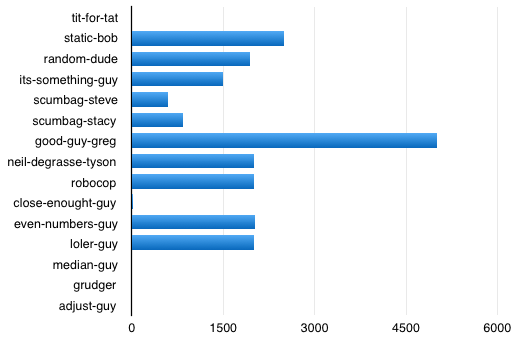
\includegraphics[scale=0.75, angle=0]{bilder/adjust-guy.png}
	\caption{Detta är bildtexten}
	\label{adjust-guy}
	\end{center}
\end{figure}
Anledningen till att good guy greg klarar sig så pass bra är att den vinner så mycket mot de strategier den faktiskt vinner mot. Det är strategier som nöjer sig med att spela tior, och inte försöker maximera sin vinst. Det gör att good guy greg inte skulle prestera särskilt bra om inte det fanns tillräckligt med sådana strategier.

\begin{figure}[htb]
	\begin{center}
	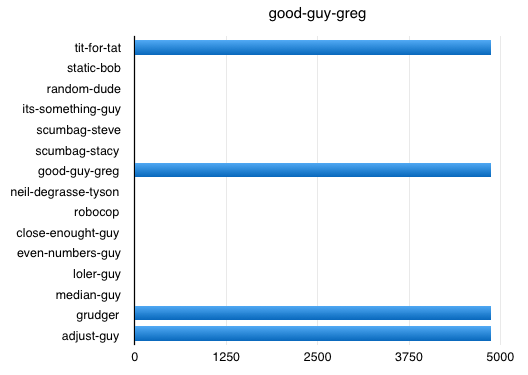
\includegraphics[scale=0.75, angle=0]{bilder/good-guy-greg.png}
	\caption{Detta är bildtexten}
	\label{good-guy-greg}
	\end{center}
\end{figure}

Median guy är en beräknande strategi. Dock spelar den bäst mot statiska strategier då den blir långsam att reagera mot strategier som alltid försöker lägga tidigare än sin motståndare. Dock kommer median guy att spela bra mot statiska strategier då den hittar vid vilket tidssteg motståndaren brukar välja och lägger sig under det. Den kommer även att spela förhållandevis bra mot strategier så som scumbag steve och scumbag stacy då median guy kommer hitta vilka värden de kör mest och sedan lägga sig under dessa.

\begin{figure}[htb]
	\begin{center}
	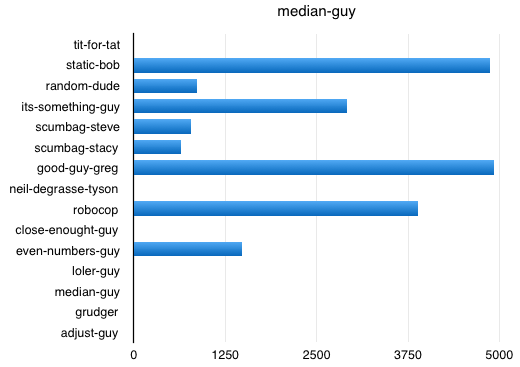
\includegraphics[scale=0.75, angle=0]{bilder/median-guy.png}
	\caption{Detta är bildtexten}
	\label{median-guy}
	\end{center}
\end{figure}


\noindent Ett intressant test som vi gjorde var att köra 10 strategier som släpper på varsitt tidssteg mot varandra flera gånger, dvs en strategi som släpper på 1, en som släpper på 2 och så vidare ända upp till 10. I detta test vann strategin som släppte på tidssteg 5 över tid. Strategi 4 och 6 hamnade på delad andra plats. Däremot så vann strategi nummer 1 över strategi nummer 5 i det “egentliga” testet. Därmet konstaterar vi att strategierna presterar väldigt olika beroende på vilka strategier som de möter.

\subsection{Projektet}
Gruppen har fungerat bra, och vi har följt tidsplanen och besvarat våra frågor. Vi kan emellertid tycka att vi skulle hittat relevant forskning i ett tidigare skede och utgå mer utifrån denna. Det var svårt att hitta artiklar som undersökt liknande frågeställningar. Vi tycker också att det var svårt att hitta vettiga problemformuleringar och frågeställningar inom just detta. Projektet startades egentligen bara med att vi diskuterade spelet och tyckte att det lät intressant att undersöka och då hamnade frågeställningarna i andrahand. Detta har inneburit att vi utvecklat vår medvetenhet gällande vad som krävs för att skriva vetenskapliga artiklar, där stor vikt skall läggas på tidigare forskning, samt formulerade av frågeställningar och hypoteser. I övrigt har projektet i sig har varit roligt att genomföra och har även gett oss ytterligare förståelse i framför allt game theory. 

\subsection{Framtida studier?}
Skall detta vara med också kanske??